\chapter{Instruction Sets}
An instruction set refers to a collection of instructions which a CPU is able to execute. This is a combination of the assembly instruction names and the machine code which the assembly language is compiled down to and which is placed into memory for execution. There are three different instruction sets which various ARM processors use. These are Thumb, Thumb-2 and ARM. A graphical representation of the instructions which are available on the various Cortex processors is shown in \autoref{fig:isa}. Here we see that the Cortex-M0 and -M1 use the Thumb instruction set while the -M3 and -M4 use the Thumb-2 instruction set. Following is a short discussion on each of the three instruction set which ARM supports. Note while reading that our processor (the Cortex-M0) only supports Thumb instructions\footnote{Not quite true. It supports 3 Thumb-2 instructions. Why 3? I don't know...}.

\begin{figure}
\centering
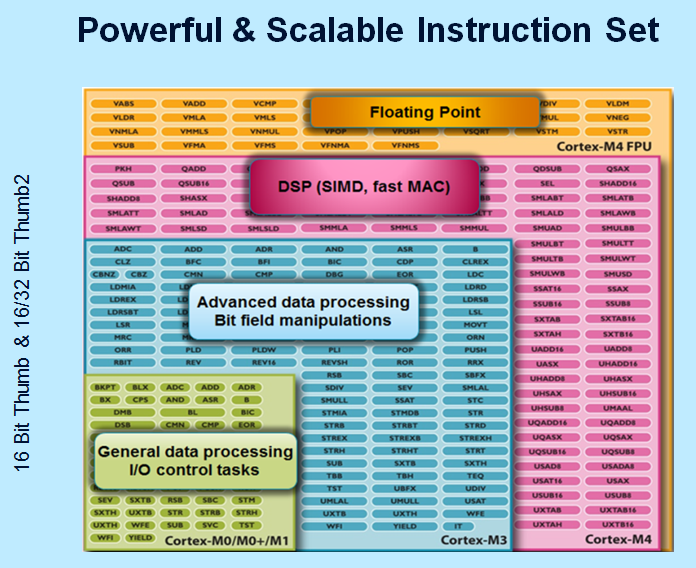
\includegraphics[width=\textwidth]{./week5/ISA}
\caption{Cortex instruction set architecture}
\label{fig:isa}
\end{figure}

\section{ARM}
The original instruction set used by ARM processors was called the ARM instruction set. This instruction set contains only 32-bit instructions. This is a powerful instruction set as almost all instruction can be conditionally executed. However, seeing as all instructions are fixed to 32 bits wide, the code density is fairly poor. This is due to comparatively simple instructions like a simple add or PC relative branch using wasteful 32 bits of flash.

\section{Thumb}
In 1994 the ARM7TDMI architecture was released which featured the Thumb instruction set. This instruction set was limited to only 16-bit instructions. Obviously these instructions were less powerful as there was less room to specify information about the actions which an instruction should perform. However for simple instructions this was not an issue and resulted in programs being much smaller. For more complicated operations multiple Thumb instructions would be needed to perform the job of a single ARM instruction. 

In order to have a combination of the performance of the 32-bit ARM instruction set and the code density of the 16-bit Thumb instruction set, an ability called \emph{interworking} was provided. Interworking allows for the CPU to switch between executing Thumb instructions or ARM instructions. This is a useful ability but introduces some additional complexity into the system.

\section{Thumb-2}
Thumb was extended to Thumb-2 in 2003. Thumb-2 allows 16-bit and 32-bit instructions to be freely mixed together without requiring interworking. Essentially Thumb-2 is a combination of the 16-bit instructions provided in Thumb as well as a whole lot of extra 32-bit instructions. This instruction set allows performance similar to the ARM instruction set while providing code density even better than Thumb. 

It's important to note the structuring of the instruction sets: As shown in \autoref{fig:isa}, Thumb-2 (Cortex-M3 and -M4) entirely contains all of the 16-bit instructions of Thumb (Cortex-M0 and -M1). Any Thumb code will run on a Thumb-2 capable processor. Any Thumb-2 code will probably NOT run on a Thumb processor. This is called backward compatibility (sort of). The ARM instruction set is completely distinct from that figure. It is a completely different instruction set which does not run on the Cortex series of processors. Processor architectures which support Thumb and ARM (such as the ARM7TDMI) require interworking to switch between the two entirely distinct instruction sets.

\section{Implementation of Interworking}
So we understand that Thumb processors can only execute 16-bit instructions. Thumb-2 processors can execute the Thumb instructions as well 32-bit instructions. ARM processors can execute a totally different set of 32-bit instructions. Some processors can run both the ARM and Thumb instruction sets. So, how do we tell one of these interworking capable processors whether an instruction is ARM or Thumb?

Firstly, note that data accesses must be aligned. Seeing as the minimum width of an instruction is 2 bytes, all instructions must be placed on  addresses which are multiples of 2. As all addresses of instructions are multiples of 2, the lsb of the PC is always a 0. The bit is therefor sort of wasted. Hence, we assign a different purpose to this bit: when it is a 0 it indicates that the instruction pointed to by the PC is an ARM instruction. When it is a 1 it indicates that the instruction pointed to by the PC is a Thumb instruction. 

Although the Cortex series of CPUs does not support the ARM instruction set, is still requires that this rule of using the lsb of the PC to specify instruction set type is adhered to. Seeing as all instructions for the Cortex series (including our CPU) are Thumb or Thumb-2, this lsb of the PC should always be set to a 1. That is why our reset vector needs to point to the address of \texttt{\_start} +1. The +1 forces the lsb to a 1 indicating that the instruction at \texttt{\_start} is a Thumb instruction. 

If a vector attempts to set the lsb of the PC to 0, the CPU will HardFault as it would be trying to execute an instruction from an instruction set which is not supported. 
